\chapter{The State of Program Induction}
\label{ch:ps-methods}

\section{The Challenge}
\label{sec:ps-challenge}

Automatic program synthesis has been a long term goal of the field of computational intelligence since its inception \cite{mannaAutomaticProgramSynthesis1971}, promising to reduce the workload of software developers by automatically solving some of the tasks they face.
And since the field's inception it has been grappling with the challenging properties of the sparse optimization space \cite{alurSyntaxguidedSynthesis2013, davidProgramSynthesisChallenges2017} that is the set of all programs in a certain programming language, namely, 
\begin{enumerate}
    \item valid error-free programs constitute an exceedingly small part of the space of possible strings, so any program synthesis algorithm that incorporates random guessing (for instance, Reinforcement Learning with random initialization \cite{suttonReinforcementLearningSecond2018}) is exceedingly unlikely to guess a valid program;
    \item a small edit in a program can result in a large difference in it's behavior (and, conversely, the same algorithm can be expressed with very different programs), hence the programs we would like to find are not clustered in any compact part of the optimization space;
    \item some of the evaluation mechanisms of programs, especially in the \emph{Reinforcement Learning from Code Execution Feedback} paradigm involve stochasticity and can yield different results for the same program.
\end{enumerate}

In other words, the search space in program synthesis is \emph{sparse}, \emph{brittle} and sometimes \emph{noisy} \cite{arnoldNoisyOptimizationEvolution2002} - all known challenges in Optimization Theory.
Methods of program synthesis can be classified by how they address these challenges.

\newpage
\section{Genetic programming}
\label{sec:gp}

\begin{figure}
    \centering
    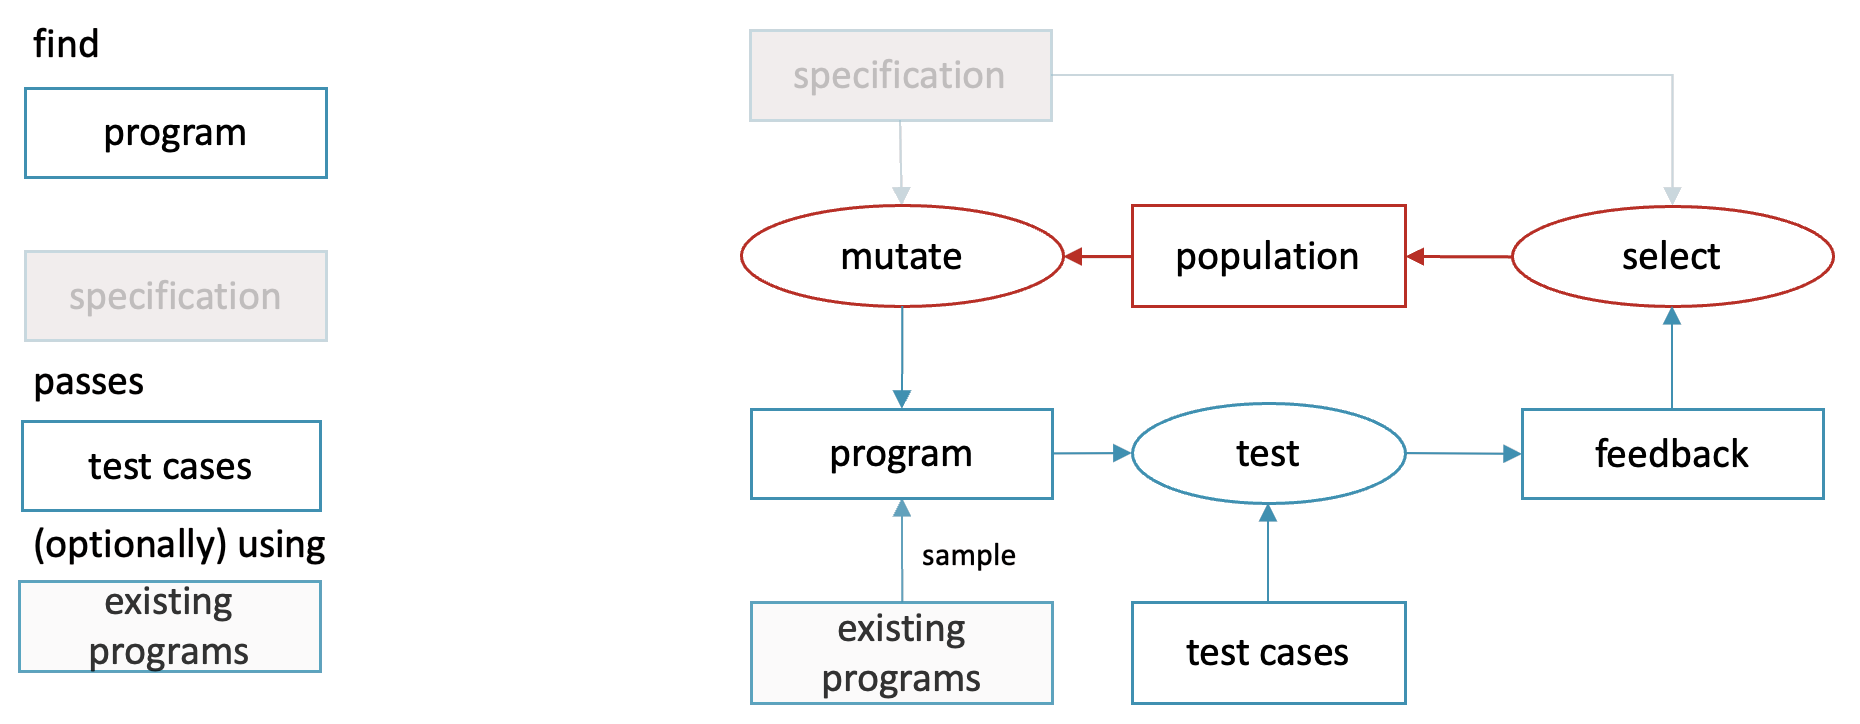
\includegraphics[width=\linewidth]{gp.png}
    \caption{Genetic Programming, schematic definition}
    \label{fig:gp}
\end{figure}

The family of optimization methods best applicable to this type of complex non-differentiable search space is \emph{genetic and evolutionary methods} - biologically inspired methods that operate on a population of candidate solutions (programs), randomly edit (\emph{mutation}) and combine (\emph{recombination}) to expand the population and the prune the population by \emph{natural selection}: removing the candidates that adhere to the specification the least.
Within program synthesis this family of methods is known as \emph{genetic programming} \cite{genprog1, genprog2, genprogast}
In an evolutionary setting, as soon as at least one (preferably several) valid program is found, initializing the population to include them drastically speeds up the search process, thus addressing the sparsity issue.
This approach is particularly powerful in a setting where some solutions are already known, but a program synthesis system can be used to search for solutions that fit the \emph{specification} even better, a setting known as \emph{genetic improvement of software} \cite{petke2018:genetic}.

Genetic programming has been successfully applied in various domains, including prediction and control \cite{dracopoulosGeneticProgrammingPrediction1997}, the synthesis of complex structures \cite{kozaHumancompetitiveApplicationsGenetic2003}, and the evolution of neural network modules \cite{degarisGENETICPROGRAMMING1990}. In the field of engineering, genetic programming has been applied to systems modeling, control, optimization, scheduling, design, and signal processing \cite{willisGeneticProgrammingIntroduction1997}. 

The biggest drawback of GP is that it requires generation and evaluation of a very high number of programs: higher than most other methods (see chapter \ref{ch:seidr}).
If evaluation of a generated program is computationally expensive, this translates directly into a very high computational cost of program synthesis.

\newpage
\section{Constrained programming languages}
\label{sec:constrainedpl}

Another way to address the complexity of the search space is to select a programming language such that the space of possible programs in that programming language exhibits less of the undesirable properties of optimization spaces.
For examples, a language where any combination of valid characters is a valid program \cite{brainfuck} eliminates a significant share of the complexity of the problem.
This family of approaches is explored in more detail in chapter \ref{ch:bfpp}, including  introduction of a novel constrained programming language for \emph{Reinforcement Learning from Code Execution Feedback}

\subsection{Domain specific languages}
\label{sec:dsl}

In some application domains it is common to express algorithms in domain specific programming languages \cite{fowlerDomainspecificLanguages2010, hudakDomainspecificLanguages1997, karsaiDesignGuidelinesDomain2014, kosarComparingGeneralpurposeDomainspecific2010, kosarDomainspecificLanguagesSystematic2016, mernikWhenHowDevelop2005} that tend to be more limited in terms of token vocabulary and grammatical complexity.
This provides the program synthesis community with a natural experiment in constraining the complexity of a language to simplify (automatic or manual) programming.
As a result, some of the most notable early positive results were in an industry standard database query language (SQL \cite{groffSQLCompleteReference2002}) \cite{liCanLlmAlready2024, yuSpiderLargescaleHumanlabeled2018} and an educational 2D robot control language (Karel \cite{pattisKarelRobotGentle1994}) \cite{metainduction}.

\subsection{Logic programming}

One domain that's particularly amenable \cite{devilleLogicProgramSynthesis1994} to solving synthesis tasks is \emph{logic programming} \cite{doetsLogicLogicProgramming1994, lloydFoundationsLogicProgramming2012}: a programming paradigm \cite{floydParadigmsProgramming2007, gorodniaiaStudyProgrammingParadigms2016, krishnamurthi13ProgrammingParadigms2019, vanroyProgrammingParadigmsDummies2009} based on formal logic. 
A program in a logic language such as Prolog \cite{clocksinProgrammingPROLOG2003} and its derivatives consists of logical relations (in the case of Prolog, Horn clauses \cite{kowalskiPredicateLogicProgramming1974}) assumed by the developer to be true, and the language interpreter runs \emph{logical inference} to establish other logical relations that must hold given the assumptions.
In other words, logic languages have built-in instrumentation for \emph{deductive logic program synthesis}: generating logic programs based on a \emph{complete specification}.
In the taxonomy introduced in section \ref{sec:tasks} this falls under \emph{code translation}.

Using tools from formal logic, such as SAT solvers \cite{gongSurveySATSolver2017} and SMT solvers \cite{reynoldsInductionSMTSolvers2015,bjornerSmtSolversFoundations2016} one can also develop search-based algorithms for \emph{inductive logic programming} \cite{cropperInductiveLogicProgramming2022, muggletonInductiveLogicProgramming1994} based on incomplete specification (programming by example) and even Reinforcement Learning from Code Execution Feedback \cite{caoGALOISBoostingDeep}.

Logic program synthesis has been applied in domains that can be described in a logic programming language such as low level hardware design \cite{siscoControlLogicSynthesis2024}, but proved difficult to generalize. 
For instance, \cite{polikarpovaStructuringSynthesisHeapmanipulating2019} proposes an extension of inductive logic programming to (more expressive) imperative programming languages that relies on the task specification (pre- and postconditions of functions to be synthesized) formulated in a logic programming language that provides the necessary structural constraints.

\newpage
\section{Grammar guided synthesis}
\label{sec:grammar-guided}

Another way to constrain the hypothesis space is to use the grammar of the programming language in question directly in the program generation process.
Since in most implementations of compilers and interpreters, the first step of program execution is building an Abstract Syntax Tree representation of the code a software tool for AST parsing is available for most programming languages.

\begin{figure}
    \centering
    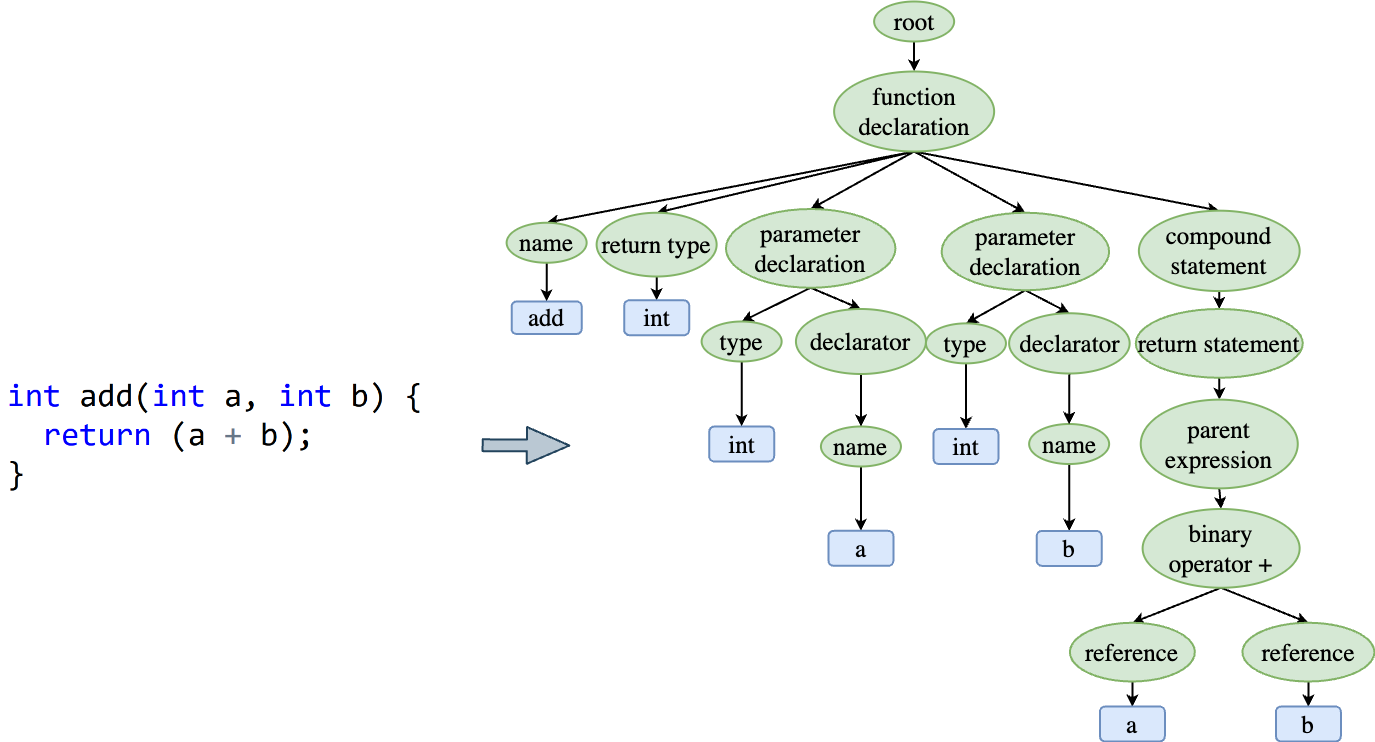
\includegraphics[width=\linewidth]{images/ast.png}
    \caption{Abstract syntax tree (AST) parser}
    \label{fig:ast-parser}
\end{figure}

When program synthesis systems output ASTs, as opposed to raw text, a large class of errors (such as forgetting a semicolon) becomes impossible. 
Grammatical rules of the language can also be used to narrow down the values a node can take based on rules associated with its parent node.
This is especially helpful in programming languages with \emph{strong typing}: structured program synthesis systems often make use of it to narrow down the space of possible identifiers that can be inserted in a location, such as a function call \cite{fengComponentbasedSynthesisComplex2017, guoProgramSynthesisTypeguided2020, oseraConstraintbasedTypedirectedProgram2019, peter-michaelProgramSynthesisTypes2015, polikarpovaProgramSynthesisPolymorphic2016}.

Research literature on structural code encoding \cite{alon2019structural,zhang2015tree}, structural code decoding \cite{jiang2021ast,zhu2019grammarcnn} and grammar-guided genetic programming \cite{bunelLeveragingGrammarReinforcement2018, manriqueGrammarguidedGeneticProgramming2009, sobaniaChallengesProgramSynthesis2020a} suggests that models that operate directly on the tree structure of the program can achieve better performance than models that operate on a sequence of tokens.
A novel approach to grammar guided program synthesis is proposed in chapter \ref{ch:tree2tree}

\newpage
\section{Human in the loop}
\label{sec:human}

Alternatively, one can narrow the scope of the problem by retaining a human developer in the loop, but supporting them with CASE \cite{caseComputeraidedSoftwareEngineering1985} tools that solve some of the subtasks involved in developing a program.

\subsection{Parametrization}

Differentiable programming \cite{blondelElementsDifferentiableProgramming2024} involves programming languages designed such that if a program computes function $f(x)$ the compiler can compute a derivative $f'(x)$. 
Machine learning can then be used to adjust all constants defined by the human developer.

Probabilistic programming \cite{gordonProbabilisticProgramming2014} is a programming paradigm where the developer is allowed to specify non-deterministic branching so that which pathway gets executed is decided randomly or externally.
The probabilities of different branches can be uniform or they can be learned in a \emph{programming by example} or \emph{Reinforcement Learning from Code Execution Feedback} fashion.
As a result, human developer outlines the options for behavior of the system at every stage and then machine learning computes which options are better suited to the data at hand \cite{gauntTerpreTProbabilisticProgramming2016}.

\subsection{Sketch completion}
\label{sec:sketching}

The paradigm of program synthesis by sketching \cite{solar-lezamaProgramSynthesisSketching2008} involves a human developer writing an approximate sketch of the desired program and a program synthesis system fills in the gaps and adds the missing details.

Today, this can be done with a \emph{programming copilot}: a software tool integrated into the text editor as a core feature or an extension, that used a pretrained language model to recommend code snippets based on the context (the code already present in the file).
At first glance \emph{copilots} may seem like a tool to accelerate typing, however, the developer can also imitate the "natural language to machine language" paradigm by describing the task at hand in a comment (or function name or docstring) and letting the copilot solve the task: see figure \ref{fig:fastinversesqrt} for an example.

\begin{figure}
    \centering
    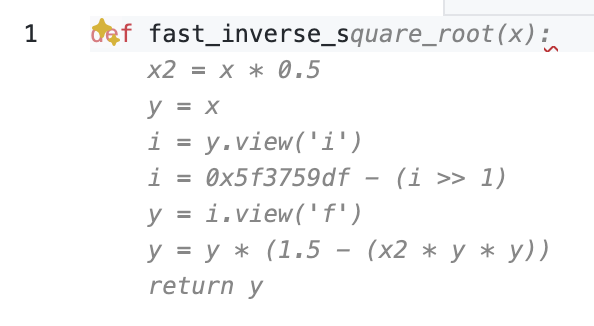
\includegraphics[width=0.35\linewidth]{images/fastinversesqrt.png}
    \caption{Github Copilot \cite{dakhelGithubCopilotAi2023, nguyenEmpiricalEvaluationGitHub2022, wermelingerUsingGithubCopilot2023} suggests an efficient inverse square root algorithm  \cite{lomontFastInverseSquare2003} before the developer finishes typing the name of the method}
    \label{fig:fastinversesqrt}
\end{figure}

Programming copilots haven proven to increase the productivity of software developers \cite{liangLargeScaleSurveyUsability2024}.
Modern copilot tools largely owe their power to unsupervised pretraining, described in section \ref{sec:pretrain}.

\newpage
\section{Unsupervised pre-training}
\label{sec:pretrain}

In \emph{unsupervised pretraining} a model is first trained on an unstructured dataset.
This model that acts as a \emph{foundation model} \cite{yangFoundationModelsDecision2023, yuanPowerFoundationModels2023, zhouComprehensiveSurveyPretrained2023} that can be adapted to solving more specific practical tasks via fine tuning \cite{panTransferLearning2020, weissSurveyTransferLearning2016a, zhuangComprehensiveSurveyTransfer2020} or composition \cite{shivakumarStudyImpactLanguage2017}.
In practice, foundation models of code are usually \emph{autoregressive} models trained to carry out \emph{next-token prediction} \cite{shlegerisLanguageModelsAre2024} - a task that does not require a structured dataset (a corpus of programs is enough) and has clear downstream applications such as programming copilots (see section \ref{sec:sketching}).
This paradigm is an attractive solution to the \emph{sparsity problem}, as it allows for a model to learn a subspace of the space of all possible strings that contains known programs in a data driven fashion.

Unsupervised pretraining can be very powerful, but it requires a large amount of \emph{data} and \emph{hardware} as well as \emph{algorithms} that can make use of available data and hardware efficiently. 
It just so happens, however, that there has recently been significant progress in all 3 areas:
\begin{enumerate}
    \item 88.12\% of the world's software developers have decided to store all of their code together in one place \cite{GithubMarketShare}. The collective wisdom of the planet's programming experts is thus pre-aggregated into a dataset that requires only minimal filtering and preprocessing \cite{kocetkovStack3TB2022} to be used for unsupervised pretraining of language models.
    \item Recent advances in hardware architectures for data parallelism (applying one mathematical operation to a set of different inputs at the same time) like GPU \cite{dallyEvolutionGraphicsProcessing2021} and TPU \cite{jouppiMotivationEvaluationFirst2018} have enabled much faster model training \cite{wangBenchmarkingTPUGPU2019}. 
    \item The Transformer architecture \cite{vaswaniAttentionAllYou2023} has replaced Recurrent Neural Networks \cite{hochreiterLongShorttermMemory1997,choPropertiesNeuralMachine2014} as the industry standard for neural sequence modeling. Unlike RNNs, the Transformer processes elements of the sequence in parallel, making better use of data parallelism afforded by GPU/TPU hardware. All the leading models in benchmarks cited below implement the Transformer with minor variations \cite{raffelExploringLimitsTransfer2023, wangGrokkedTransformersAre2024, geipingCrammingTrainingLanguage2022, liuBetterFewShotFinetuning2023, liuSwinTransformerV22022, rabeSelfattentionDoesNot2022, soPrimerSearchingEfficient2022, sunLengthExtrapolatableTransformer2022, xieResiDualTransformerDual2023, burtsevMemoryTransformer2021a, dingCogViewMasteringTexttoImage2021, dingERNIEDocRetrospectiveLongDocument2021, henryQueryKeyNormalizationTransformers2020, heRealFormerTransformerLikes2021, huangAttentionAttentionImage2019, luUnderstandingImprovingTransformer2019, nguyenTransformersTearsImproving2019, parisottoStabilizingTransformersReinforcement2019, PathwaysLanguageModel, pressImprovingTransformerModels2020, pressTRAINSHORTTEST2022, shazeerFastTransformerDecoding2019, shazeerGLUVariantsImprove2020, shazeerTalkingHeadsAttention2020, shleiferNormFormerImprovedTransformer2021, sukhbaatarAugmentingSelfattentionPersistent2019a, wangCrossFormerVersatileVision2021, zhangRootMeanSquare2019, zhaoExplicitSparseTransformer2019, ZhiXuJiXingDaiMaGaiJinTransformerZiZhuYiLiJiZhiJiHuBuZengJiaJiSuanLiang}.
\end{enumerate}

As a result of this trifecta of antecedents, unsupervised pretraining has enabled significant progress in code translation settings such as \emph{natural language to machine language} \cite{chenEvaluatingLargeLanguage2021, conala, guoContentEnhancedBERTbased2020, hallerPECCProblemExtraction2024, hendrycksMeasuringCodingChallenge2021, honarvarTurbulenceSystematicallyAutomatically2025, huQualityFlowAgenticWorkflow2025, jimenezSWEbenchCanLanguage2024, leiPlanningDrivenProgrammingLarge2025, liEnablingProgrammingThinking2023, liExploringEffectivenessLlms2023, psb2, solimanMarianCGCodeGeneration2022, the-crypt-keeperThecryptkeeperCanaicode2025, zhuoBigCodeBenchBenchmarkingCode2024} and even human-comparable performance in coding competitions \cite{liCompetitionLevelCodeGeneration2022,openaiCompetitiveProgrammingLarge2025}.
However, for the purposes of RLCEPS

\begin{highlight}
    Reinforcement Learning from Code Execution Feedback is still a nascent field with no method available for us to deploy in a patient simulator.
\end{highlight}

Chapters \ref{ch:bfpp}-\ref{ch:seidr} are dedicated to developing such a method.